\subsection{Building an Intuition of the Transistor}

We have in the previous chapter presented all the necessary information to understand the basic structure of NE1's rockstar: the transistor. Specifically, we'll be looking at the \textit{Metal-Oxide-Silicon-Fielf-Effect-Transistor}, commonly called \textit{MOSFET}, which is a particular type of Transistor, extremely common in industry. There exists other types of transistors that we don't look at in this course, such as the BJT (Bipolar Junction Transistor), as well as many others. The currents in these devices comprise either positively-charged holes, negatively-charged electrons, or both holes and electrons. The BJT is called a bipolar device because the current in the transistor consists of both types of carriers, electrons and holes. The MOSFET is called a unipolar device because the current has only one type of carrier, either holes or electrons.
All transistors have at least 3 terminals (often 4). Though they all exhibit similar behaviours, some differences make them more useful in some applications. This section is mostly about developping an intuition about the transistor structure and function. We will get into the specifics of operation in the next section and derive the precise equations that best describe its behaviour.  

The main purpose of transistors is to control the flow of current from one node based on the potential at another node: by controlling voltage, you control current. Once again, let's start with some fluid analogy to build intuition on the transistor. 

\subsubsection{Understanding the transistor idea with Hydraulic Analogy}

\begin{figure}[H]
    \centering
    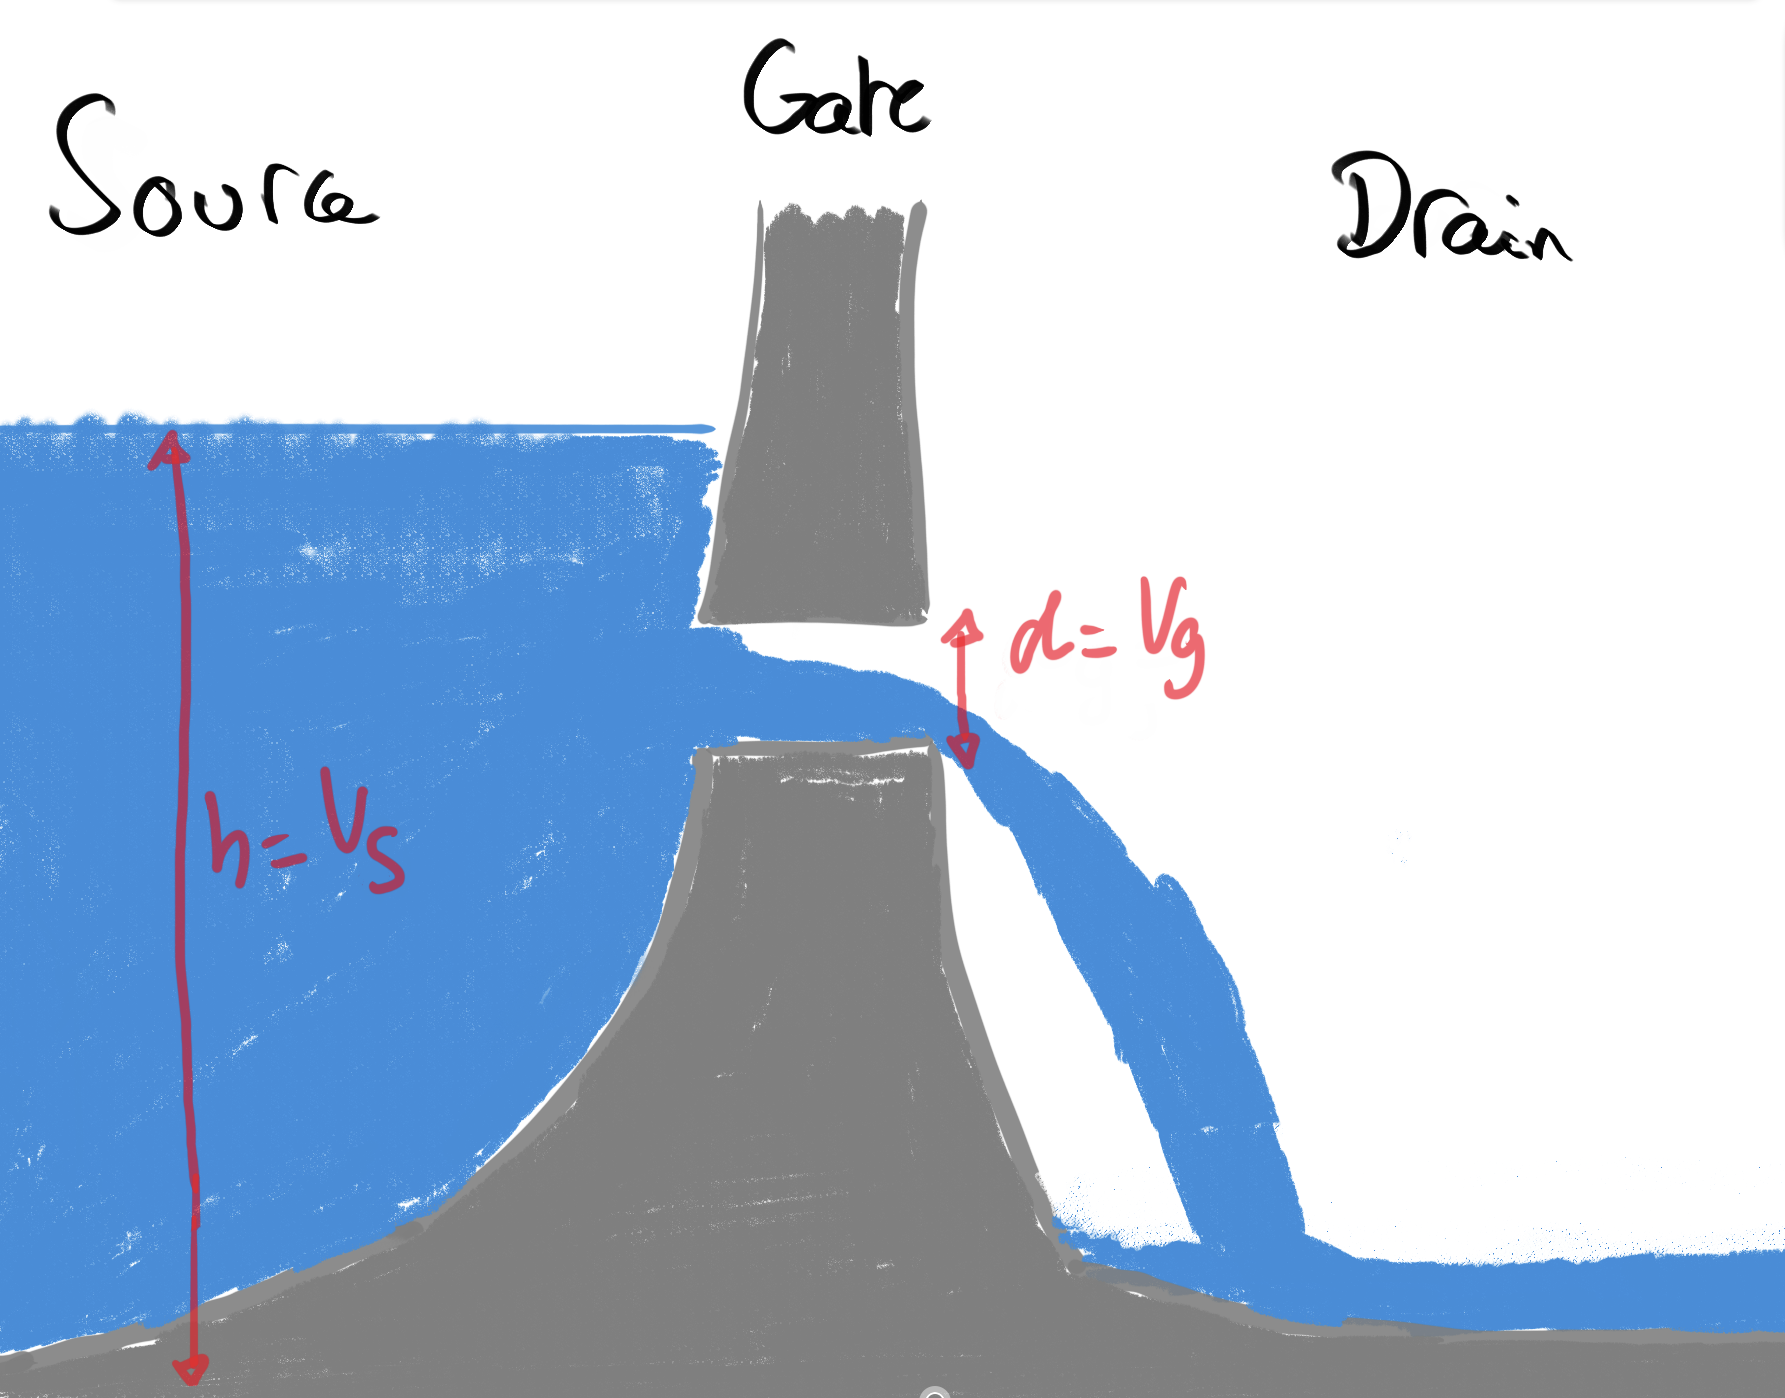
\includegraphics[width=0.75\linewidth]{../../Figures/Transistor analogy.png}
    \caption{Water analogy to understand the transistor. My personnal drawing, inspired by a bunch of drawings I saw online.}
    \label{fig:Transistor analogy}
\end{figure}

I never managed to find the right drawing for what I was trying to convey, so I drew my own.
Things are pretty self explanatory on the figure: there is water in some sort of reservoir, that we can call \textbf{source}, and no water in the \textbf{drain}. Let's imagine that the water in the source doesn't run out, i.e. each molecule that eventually flows out is brought back through some external supply not represented here - so $h$ stays fixed.

Now, remember from chapter 0 that because water is at a certain height $h$ compared to the ground (where the drain is), there is some \textit{potential difference} between the source and the drain - this is a very important point. There is also separation between the source and the drain, called the \textbf{gate}. We can now bring some energy to open this gate (as it needs to be lifted) and open it up to a certain level $d$. The level at which we open it will determine the extent by which water flows from the source to the drain. Now imagine that the drain gets full up to the same level as the source - even if the gate is opened, there is no net flow between the source and the drain. So we need \textbf{both} an opening of the gate \textit{AND} a potential difference between the source and the drain in order to generate flow. 

The way we open the gate also has an impact on the way water flows. Imagine that $d$ is small compared to $h$, then you have a small flow. The more you open the gate (increasing $d$), the more things flow. The water flow (in our analogy) is \textbf{exponentially} dependant on the gate opening. But if we open the gate to some high $d \geq h$, well water flow does not really depend on $d$ anymore\footnote{Remember that there is a constant supply of water in the source so that $h$ stays constant}! Past this \textit{threshold}, the gate is opened and water flows independant of how much bigger our opening is.

It should be clear the kind of dynamics that we're trying to put in evidence here: when we have a potential difference between the source and the drain, water wants to flow. This water will flow if we open the gate, and the nature of the flow will change depending on how large the gate opening is. This is the basic idea of a transistor.

One thing that need to be added to the analogy: water evaporates. It is possible when the gate is open that water from the drain gets into the source, but this is in such small quantity that it is often negligible - though it is still there! The higher the potential difference between the source and the drain, the lower the chances that water evaporates from the drain to the source. This is the idea of forward and reverse flow, which is important in transistors as we will see. When the potential difference between source and drain is high, forward flow is overwhelmingly dominant, when the potential difference is very small, the reverse flow should also be considered to some extent, in particular conditions.  


\subsubsection{Understanding Sub-threshold Current using Boltzmann Distribution}
\textbf{nFET transistor without connecting to voltage supply}
\begin{figure}[H]
    \centering
    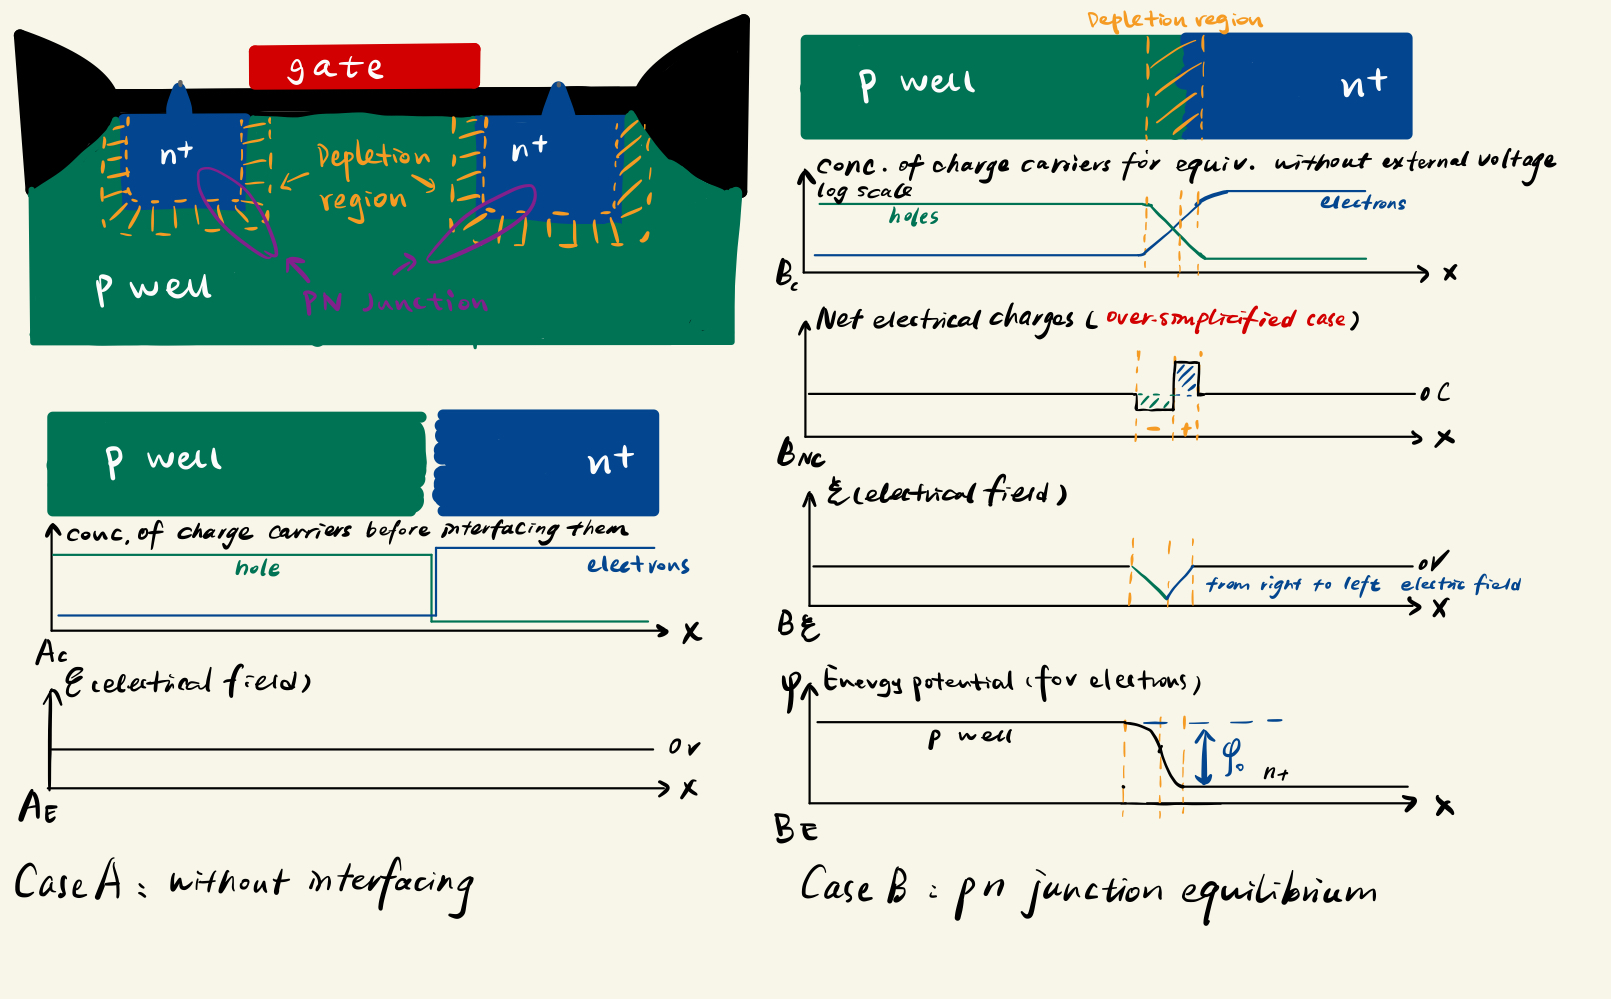
\includegraphics[width=0.9\linewidth]{Figures/PNjunc4Transistor_1.jpeg}
    \caption{An illustration of a nFET transistor without attaching external voltage to its terminals. And case A and case B help explains how depletion region between highly doped n type node with p well is formed, and what properties it has, e.g., electrical field and energy potential. The depletion region is then oversimplified to be considered as have exactly no free charge carriers for further calculation. Figure drawn by Wencan Huang}
    \label{fig:342_transistor_1}
\end{figure}

Without loss of generality, detailed physics and math expressions are deliberately omitted and any curious readers can refer to semiconductor physics textbook or Caltech online courses. Knowing nothing about those details is totally okay for succeeding in this course, however, it is necessary to understand the general idea presented in this section. 

When there are no external voltage difference attached to nFET transistor's terminals, the depletion region between p well substrate and two n type nodes is formed due to diffusion and reaches equilibrium due to the electrical field formed during diffusion as is indicated in the figure \ref{fig:342_transistor_1} for electrical field in plot \(B_\epsilon\). 

For simplicity, take n type side for consideration and the same analysis can be followed for the p well side. The diffusion effect on the n type tries to diffuse n type free charge carriers - electrons - among the whole p-n junction. However, as electrons diffuse into p well side, they will leave net positive charge in n type side through fixed positive ions which lose valence electrons, and cause net negative charge in p well side through contributing electrons to group III element. As a result, an electrical field is formed counterbalancing the diffusion of electrons towards p well side, and the equilibrium of diffusion is reached as drawn in figure \ref{fig:342_transistor_1} for concentration of free charge carriers in plot \(B_C\). 

Due to the effect as mentioned in the paragraph above, with oversimplified mathematical models, we assume that within the depletion region, the charge density is constant as shown in plot \(B_{NC}\). Based on this assumption, we gain the consequent plots for electrical field and energy potential for electrons. In general, for silicon transistors, the potential gap \(\phi_{0}\) is around 0.7V. 

\bigskip
\noindent\textbf{nFET transistor connecting to voltage supply without considering \(V_{g}\) yet}

For neuromorphic engineering I, what we care most is transistor's operation in sub-threshold region, i.e., \( 0 < V_{gs} < V_{thr}\) \textcolor{red}{add the hyperlink to related sections here and ensure the symbols are consistent}. Besides, a nFET transistor is only used with source-p well and drain-p well reverse biased. And the rest part will only consider under such circumstances. 

\begin{figure}[H]
    \centering
    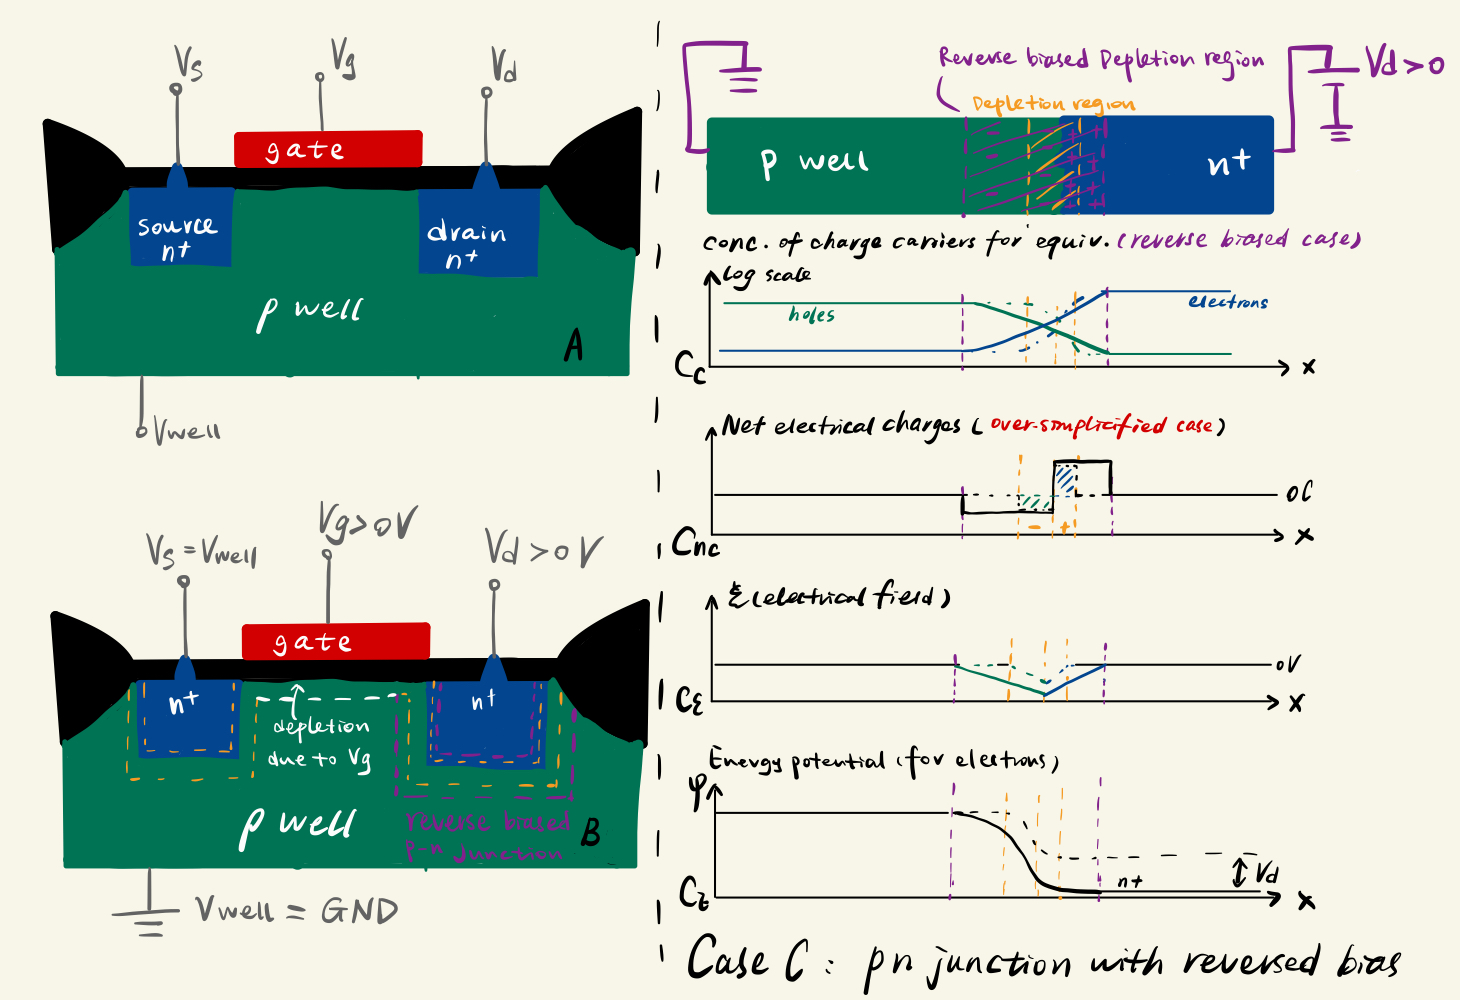
\includegraphics[width=0.9\linewidth]{Figures/PNjunc4Transistor_2.jpeg}
    \caption{A illustrates how a nFET transistor is typically used by providing four voltage. B shows what are typical voltages applied for neuromorphic usage (note: for sub-threshold, \(V_{gs}<V_{thr}\)) . Case C compares how depletion region properties changes when the p-n junction is reverse biased without considering the effect of \(V_g\) in solid line with case B in dashed line. Figure drawn by Wencan Huang}
    \label{fig:342_transistor_2}
\end{figure}

Figure \ref{fig:342_transistor_2} demonstrates how nFET transistors are connected to different voltage in general and illustrates how depletion region changes upon voltage difference acting on drain or source. To understand step by step, case C deliberately ignored the effect introduced by \(V_{g}\) through a simplification assuming that \(V_{g} = 0V\). In this case, the p-n junction between highly n doped drain and p well is reserve biased, which expands the depletion region. While since the p-n junction between source and p well has no voltage difference, its situation is the same as in case B. 

The properties changed for p-n junction between drain and p well is shown in the four plots, and one important information is that the energy potential for electron in drain is dropped exactly by the supplied voltage \(V_d\). And this is because that it is this supplied voltage expands depletion region when there is no external voltage applied, and thus the potential change for electron should be exactly the same value. And recalling the potential gap \(\phi_{0}\) introduced in figure \ref{fig:342_transistor_1}, the energy potential gap between drain and p well now becomes \(\phi_{0}+V_{d}\). 

\bigskip
\noindent\textbf{nFET transistor connecting to voltage supply considering \(V_{g}\)}

To discuss the effect due to gate voltage, it is necessary to understand the effective capacitance due to depletion region. More mathematics can refer to later sections. \textcolor{red}{add the hyperlink to related sections here and ensure the symbols are consistent}.

\begin{figure}[H]
    \centering
    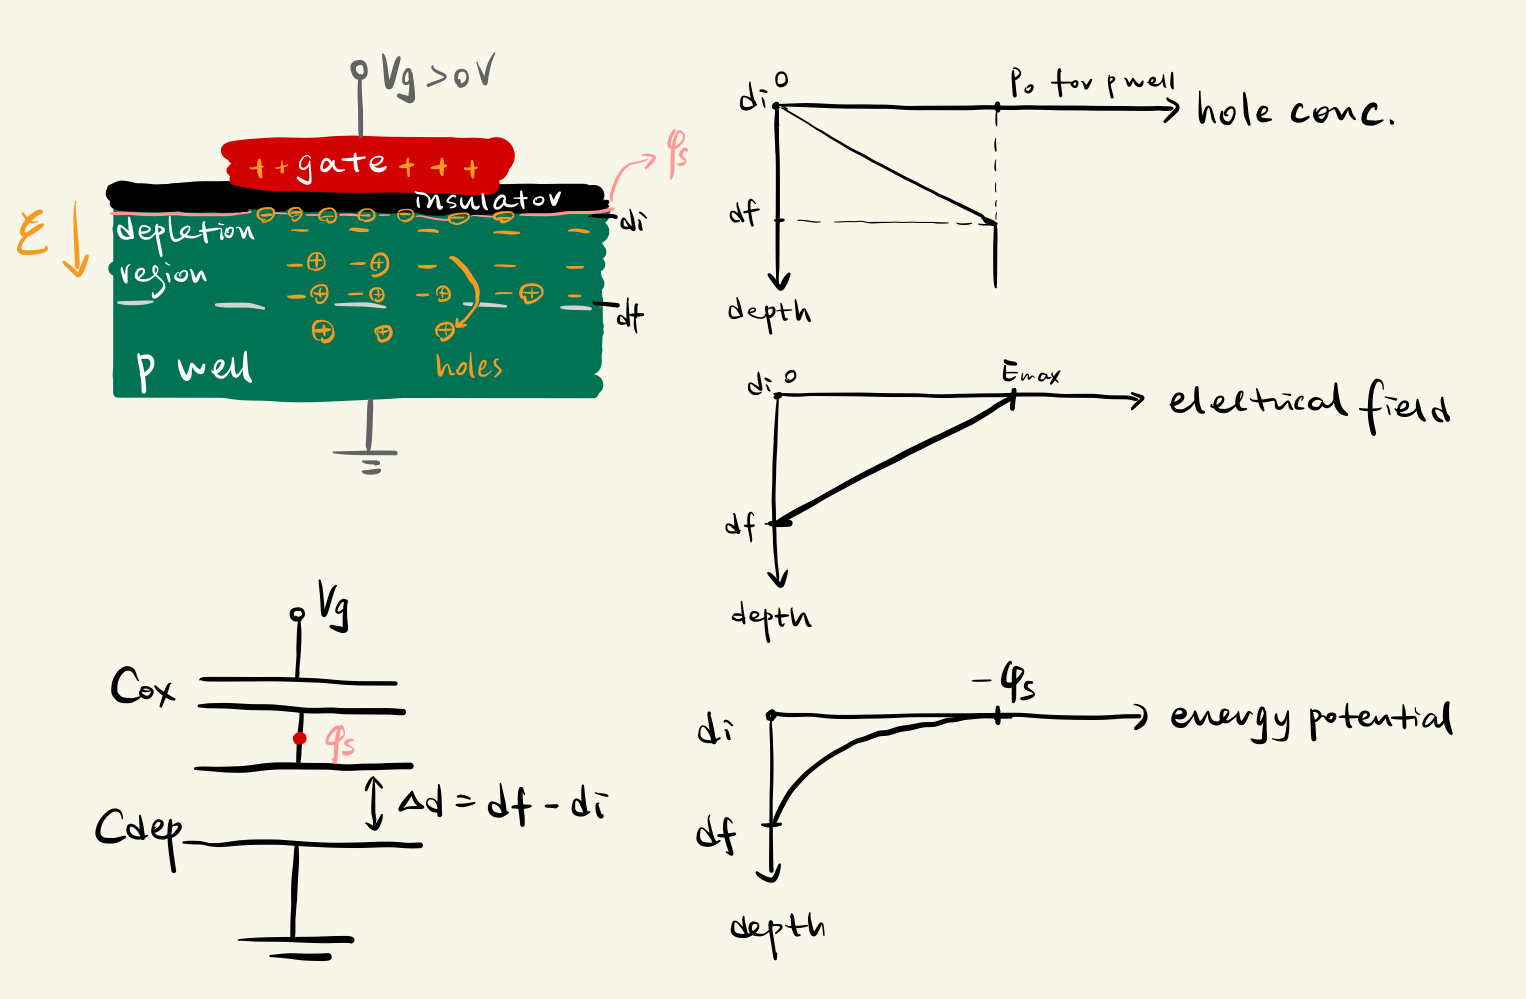
\includegraphics[width=0.9\linewidth]{Figures/PNjunc4Transistor_3.jpeg}
    \caption{A illustrates how a nFET transistor is affected by \(V_{g}\) as a capacitor. The hole concentration in the first plot changes linearly in log scale according to diffusion - drift balance just as in figure \ref{fig:342_transistor_1}. And the energy potential for electron in the third plot is along the negative direction with \(\phi_s\) defined as positive. Figure drawn by Wencan Huang}
    \label{fig:342_transistor_3}
\end{figure}

Along the direction of vertical section, from gate to p well as shown in figure \ref{fig:342_transistor_2} B without considering drain and source, nFET transistor in this case can be considered equivalent to two serial capacitor - one constant capacitor due to the insulator layer, and one causal capacitor due to \(V_{g}\). 

As is shown in three plot in figure \ref{fig:342_transistor_3}, the hole concentration in p well can be considered to change exactly the same as in p-n junction in figure \ref{fig:342_transistor_1}. With the same simplification as in case A, we can consider the charge density within the depletion region are exactly the same. As a result, this causes a gradual linear change in electrical field through the depletion region, which in terms gives a parabolic change in energy potential, which gives \(\phi_{s} \propto \delta d^2 \), i.e., \(d \propto \sqrt{\phi_{s}}\). 


However, currently we use the term \(\phi_{s}\) without identifying what this term is. As is demonstrated by the figure of two capacitor, \(\phi_s\), surface potential refers to the potential for electrons just below the insulator, and its value is mutually determined by \(V_g\) and \(C_{dep}\) which is caused by \(V_g\). 

And using the model of two capacitor without considering the change in \(\Delta d\) and \(C_{dep}\), the change in \(V_g\) and \(\phi_s\) should satisfy: \(C_{ox}(\Delta V_g - \Delta \phi_s) = C_{dep}\Delta \phi_s\), which gives \(\dfrac{d\phi_s}{dV_g} = \dfrac{C_{ox}}{C_{ox}+C_{dep}}\). Since when \(V_g = OV\), \(\phi_s = OV\), and for subthreshold region \(\Delta V_g\) is small, we can assume that \(\phi_s = \kappa V_g\) with \(\kappa := \dfrac{C_{ox}}{C_{ox}+C_{dep}}\). 

In the above paragraphs, we consider how \(\phi_s\) changes without considering changes in \(C_{dep}\), and this only holds when \(C_{dep}\) changes negligibly with respect to changes in \(V_g\). Therefore, we intuitively explain why this is true. 